\section{Reproducibility, notation, and proof scope}\label{app:implementation}
The accompanying directory contains the LaTeX source, original data files, extracted panels, and offline Python programs. The example program reproduces the deterministic theoretical illustrations. The empirical program reproduces the historical-sample figures and calibration outputs using NumPy, SciPy, and Matplotlib. A separate decomposition program compares the saved independent-chain and calendar-fit errors. It performs monotone scalar inversion and linear programming, without simulating paths. The input hashes identify the exact versions of the three prepared datasets used in the analysis.

The synthetic example uses exact Gaussian cash prices. Its background volatility remains constant through the end of accrual. Discount factors and forward-measure means are fixed at their generating values. Its bounds are exact for the extracted variance observations; the additional structural restrictions tying those fixed means to candidate variances are not imposed. The empirical analysis uses the normal diagnostic \eqref{eq:normalproxy} and the smile-based ATM proxy \eqref{eq:smileatm}, with the selection rule and background schedules stated in Section~\ref{sec:empirical}. Puts and calls enter according to the selected out-of-the-money side; no European parity equation is imposed on the American settlements.

The data provenance records source locations, units, strike decoding, contract mappings, archive coverage, and missing inputs. Calendar ranks use only meetings after the valuation date and no later than the last retained expiry. The analysis is repeated separately by date; it imposes neither temporal smoothing nor a physical-measure time-series law. Market observations across dates share contracts and are not treated as independent statistical replications.

For the minimum-error calculation, all strike intervals at an expiry are intersected before the feasibility problem is solved. Bisection terminates when the premium-tolerance bracket is below 0.0001 bp. The code verifies price inversion, the linear constraints at both optimized endpoints, and price residuals at the reported feasible tolerance. The local calendar-hedge sensitivity is also checked by finite differences. Infeasible training sets do not generate prediction intervals. No held-out price is used to choose its training tolerance.

\subsection{Smile, loading, and exercise calculations}\label{app:empiricalmethod}
The extension program fits the mixture \eqref{eq:mixture} separately by chain. To scale the optimization, divide displacements and standard deviations by the closest-strike implied normal standard deviation, floored at 1 bp. In these units constrain $d\in[-2,2]$ and $\log s_j\in[-3,1.5]$. Use starts $(0,0,0)$, $(0.5,-0.5,0.2)$, and $(-0.5,-0.5,0.2)$ for $(d,\log s_1,\log s_2)$, retaining the converged solution with smallest squared price residual. All 555 standard fits converge. These bounds and local optimization are part of the interpolation specification; global optimality or identification of mixture parameters is not asserted. The omitted-closest-strike calculation uses the same starts and bounds and never fits to the withheld premium. Its scale uses only training strikes.

The loading calculation integrates the maturity average analytically and uses 20-point Gauss--Legendre quadrature in shock time, separately on each background cell. For every candidate shape, weighted nonnegative least squares gives the date-specific allocation. The original 37-shape grid includes the parallel case $\chi=0$. The free-long-end grid uses
\begin{align*}
\kappa&\in\{0.25,0.5,0.75,1,1.25,1.5,2,3,4\},\\
\chi_1&\in\{0,0.5,1,2,4,8,12,16\},\qquad
\chi_2\in\{0,0.25,0.5,1,2,4,8\}.
\end{align*}
Removing eight duplicates of the parallel shape leaves 496 shapes. Its pure-hump subset has 64 distinct shapes. When the selected amplitude reaches a grid boundary, the sensitivity grid uses both amplitudes in $\{0,1,2,4,8,12,16,24,32,48,64\}$ and the same decay grid: 1,081 distinct shapes. This is a discrete grid check, not a continuous global optimum or parameter confidence region. Shape selection and date-specific fitting exclude all S3 observations in both searches. The additional family itself was chosen after the original S3 failure, so that comparison reuses an examined sample. The subsequent all-product interval analysis is separate; its fit counts and ranges are not held-out results. Shape-profile endpoints are the smallest lower and largest upper endpoints across feasible shapes on the original grid.

The American tree uses increments $-\sqrt{3\cV_{\rm ATM}/n}$, $0$, and $+\sqrt{3\cV_{\rm ATM}/n}$ with probabilities $1/6$, $2/3$, and $1/6$. Each step discounts by $D^{1/n}$. Backward induction takes the maximum of discounted continuation and intrinsic value for the American claim, and continuation alone for the European claim. Their difference on the same grid isolates exercise value. At zero discount rate the code checks that the exercise premium vanishes. The European price is also compared with the analytic normal formula. This benchmark holds the normal variance rate and discount rate constant and does not model scheduled jumps.

For the empirical proxies, uncertainty about smile interpolation, exercise, the forward-measure mean, and the loading shape is not combined into a statistical confidence set. The reported intervals answer explicit sensitivity questions conditional on those choices. A listed-contract structural estimation would require a joint smile and exercise model, the appropriate stochastic discounting, and a convention-matched independent curve. Neither the mixture fit nor its good local interpolation test supplies those additional ingredients.

\subsection{Conditional ranges under the original hump}\label{app:shapeprofile}
Using all 256 standard and same-expiry midcurve ATM observations gives feasible sets conditional on the original hump $(\chi,\kappa)=(4,0.75)$. The median minimum ATM-price allowance drops from 3.319 bp under parallel loading to 1.136 bp with the hump and constant background, 1.078 bp with 90-day cells, and 0.936 bp with expiry-gap cells. At a 1 bp allowance, these three humped specifications fit respectively 2, 5, and 9 of the fourteen dates; no parallel specification fits a date.

On 22 July, the first date fitting all three humped backgrounds at that allowance, the September-meeting ranges are $[88,550]$, $[0,550]$, and $[0,1038]$ bp$^2$ for constant, 90-day, and gap backgrounds. The January 2027 ranges are $[414,973]$, $[378,2113]$, and $[314,2514]$ bp$^2$. Same-expiry windows now add background information: with expiry-gap cells the matrix rank rises from 7 under parallel loading to 12 out of 15 columns under the hump. In contrast to the standard-only parallel experiment, assigning each increment to its own background cell no longer makes all meeting lower bounds vanish.

Conditioning on an estimated shape can overstate this information. Taking the union of the constant-background feasible sets over the entire grid gives September range $[0,550]$ and January range $[0.16,973]$ bp$^2$ on 22 July. Only two grid shapes fit that date within 1 bp. The tiny positive January endpoint is specific to the finite grid; it is not a positive bound over all smooth loadings. These original-hump calculations illustrate the effect of conditioning on a shape. They are separate from the free-long-end prediction comparison in Section~\ref{sec:humpfit}.


\subsection{Exact ATM calculation for discrete meetings}\label{app:additivity}
This synthetic example isolates the observation transform. It specifies an arithmetic futures martingale directly, rather than claiming that binary jumps satisfy the Gaussian rate model. Let meetings occur at $T_i=i/8$ year, let $\epsilon_i$ be independent symmetric signs, and let $W$ be an independent Brownian motion. At expiry $S_n=n/8$, put
\[
X_n=25\sum_{i=1}^n\epsilon_i+\sigma W_{S_n},\qquad
D_n=e^{-0.04S_n},\qquad n=1,\ldots,8.
\]
Displacements are in bp and $\sigma$ in bp per square-root year. Its true variance is $625n+\sigma^2S_n$. Conditional on $k$ positive outcomes, the displacement is normal with mean $\mu_{nk}=25(2k-n)$ and standard deviation $s_n=\sigma\sqrt{S_n}$. Thus its exact European ATM price is
\[
\frac{C_n}{D_n}=2^{-n}\sum_{k=0}^n\binom nk
 \left[\mu_{nk}\Phi(\mu_{nk}/s_n)+s_n\varphi(\mu_{nk}/s_n)\right],
\]
using $(\mu_{nk})^+$ when $s_n=0$. Define $\cV_{{\rm ATM},n}=2\pi(C_n/D_n)^2$ and $\cV_{{\rm ATM},0}=0$.

The increments are independent and identically distributed, so additivity of the proxy would imply $\cV_{{\rm ATM},n}=n\cV_{{\rm ATM},1}$. The resulting ATM-price error is
\[
D_n\sqrt{n\cV_{{\rm ATM},1}/(2\pi)}-C_n.
\]
Alternatively, an unconstrained meeting-by-meeting fit with the correct background variance rate would infer
\[
\widehat v_n=\cV_{{\rm ATM},n}-\cV_{{\rm ATM},n-1}-\sigma^2/8.
\]
All these increments are nonnegative in the four computed scenarios, so an exact nonnegative calendar fit is possible. Yet $\widehat v_n$ need not be 625 bp$^2$.

\begin{center}\small
\begin{tabular}{rrr}
\toprule
$\sigma$ (bp/$\sqrt{\mathrm{year}}$) & Maximum price error (bp) & Range of $\widehat v_n$ (bp$^2$)\\
\midrule
0 & 7.697 & $[0,1246.4]$\\
25 & 5.005 & $[351.6,904.6]$\\
50 & 2.323 & $[549.3,770.4]$\\
100 & 0.532 & $[616.6,672.3]$\\
\bottomrule
\end{tabular}
\end{center}
Figure~\ref{fig:additivity} displays the errors and two allocation examples. Even the largest background in the table leaves a maximum price error above 0.25 bp. In the Gaussian control, replacing each sign jump by an independent centred normal variable of variance 625 makes the ATM proxy equal the true variance at every expiry; both errors then vanish. The discrete example demonstrates a possible structural error, not its empirical size in the settlement panel.

\begin{figure}[ht]
\centering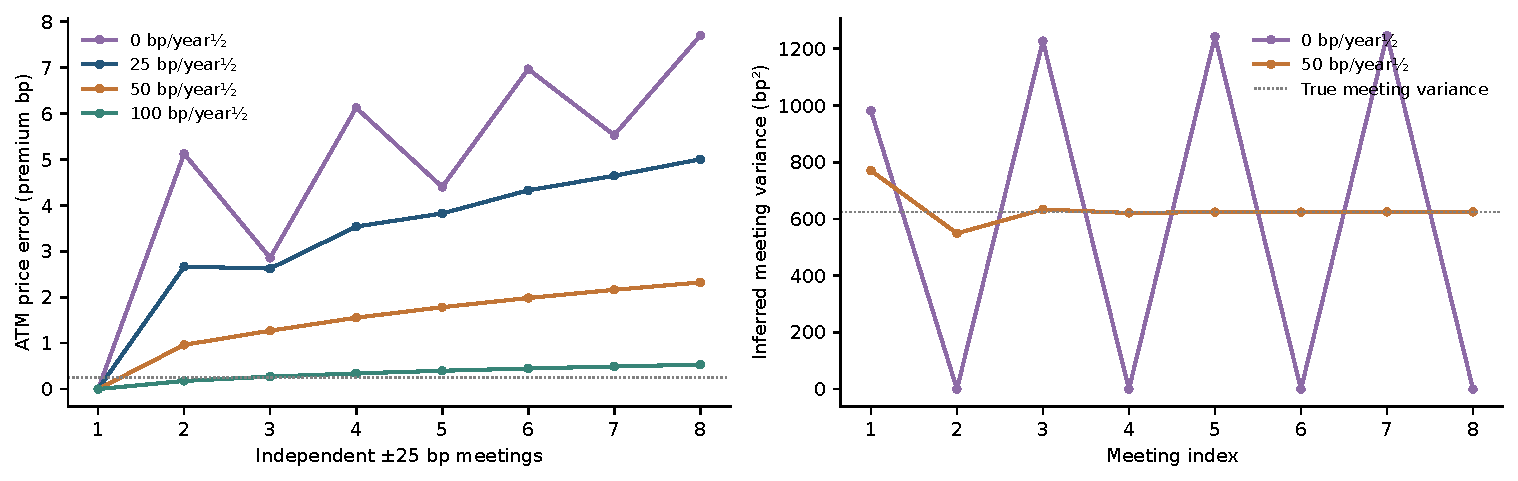
\includegraphics[width=\textwidth]{figures/atm_additivity.pdf}
\caption{Independent $\pm25$ bp meetings with Gaussian background. Left: ATM-price error from adding the identical one-increment ATM proxies; the dotted line is 0.25 bp. Right: meeting variances inferred by fitting each expiry exactly and subtracting the known background. Every actual meeting has variance 625 bp$^2$ (dotted line).}\label{fig:additivity}
\end{figure}

\FloatBarrier
\subsection{Second-moment and front-loading sensitivities}\label{app:finalsensitivities}
\paragraph{Second moments.}
The fitted mixture has mean zero and variance
$\widehat{\cV}_{2,\ell}=d_\ell^2+(s_{1,\ell}^2+s_{2,\ell}^2)/2$.
Unlike the ATM proxy, this is the variance of the fitted law. Its use still extrapolates that law beyond the observed strikes, and fitting separate expiry laws does not establish independent increments or a common pricing measure. We apply the parallel calendar equation to these moments as a companion sensitivity calculation.

For comparability, retain the numerical ATM-price allowances $\varepsilon_\ell$ in \eqref{eq:robustallowance}. Multiplying the entire centred mixture displacement by a positive scalar multiplies its ATM price by that scalar and its second moment by its square. Thus an ATM-scale perturbation induces a moment interval. Widen that interval by an additional relative allowance $\zeta\in\{0,0.10,0.25,0.50\}$:
\begin{equation}\label{eq:momentinterval}
(1-\zeta)\widehat{\cV}_{2,\ell}
 \left\{\left(1-\frac{\varepsilon_\ell}{\widehat c_{{\rm ATM},\ell}}\right)^+\right\}^2
\ \leq\ (\mathsf A\theta)_\ell\ \leq\
(1+\zeta)\widehat{\cV}_{2,\ell}
 \left(1+\frac{\varepsilon_\ell}{\widehat c_{{\rm ATM},\ell}}\right)^2.
\end{equation}
The values of $\zeta$ are sensitivity scenarios, not estimated tail-error bounds or confidence levels. The numerical $\varepsilon_\ell$ are reused as scale allowances; their exercise and mean components are not recalculated under the mixture law. This experiment does not transfer the Gaussian seed-containment argument to a different pricing model.

On 18 June the ratio $\widehat{\cV}_{2,\ell}/\widehat{\cV}_{{\rm ATM},\ell}$ ranges from 0.892 to 1.392 across seven expiries. With $\zeta=0$, constant and 90-day backgrounds are infeasible; expiry-gap background is feasible and permits zero for both headline meetings. Table~\ref{tab:momentcheck} reports the wider scenarios. At $\zeta=0.50$, all three specifications permit zero for both meetings. The positive constant-background bounds at $\zeta=0.10$ therefore demonstrate a conditional contrast between backgrounds, not distribution-free positive lower bounds.

\begin{table}[ht]
\centering\small
\begin{tabular}{rlrr}
\toprule
Extra allowance & Background & 16 September 2026 & 27 January 2027\\
\midrule
10\% & Constant & $[275,1058]$ & $[1549,4229]$\\
 & 90-day cells & $[0,1343]$ & $[0,5125]$\\
 & Each expiry gap & $[0,1470]$ & $[0,5125]$\\
25\% & Constant & $[0,1552]$ & $[91,5740]$\\
 & 90-day cells & $[0,1789]$ & $[0,6487]$\\
 & Each expiry gap & $[0,1895]$ & $[0,6487]$\\
\bottomrule
\end{tabular}
\caption{Mixture-second-moment meeting-variance ranges on 18 June under \eqref{eq:momentinterval}, in bp$^2$, rounded to the nearest integer. These are sensitivity ranges for an extrapolated second moment.}\label{tab:momentcheck}
\end{table}

\paragraph{Flattening the front of the loading.}
Write the selected free-level loading as a function of maturity distance,
$\phi(\tau)=1+18\tau e^{-1.5\tau}+8(1-e^{-1.5\tau})$.
For a cutoff $h\geq0$, replace it by $\phi(\max\{\tau,h\})$ and divide by its value at $\tau=1$. This keeps the tail unchanged up to a common scale and makes the front constant. We rebuild the 22 July all-product exposure matrix with expiry-gap background cells; there are 17 observations and 15 parameter columns. No coefficients are refitted. Maturity averaging is analytic, and shock-time integration is split where a window crosses the cutoff.

The ranks for $h=0,0.5,1,1.5$ years are all 12. In the same ACT/360 parameter coordinates, the smallest nonzero singular value divided by the largest is respectively $4.05\times10^{-4}$, $7.64\times10^{-5}$, $7.14\times10^{-5}$, and $1.51\times10^{-6}$. Removing the first half-year's slope weakens this relative sensitivity by a factor of 5.3 without destroying exact rank. Setting $h=4$ years flattens the entire observed exposure domain, reproduces the parallel matrix, and reduces rank to 7. The rank increase therefore does not depend exclusively on the steep front, but its numerical strength is sensitive to that part of the curve. These singular values compare the stated coordinate scaling; they are not invariant measures of statistical precision.\FloatBarrier

\subsection{Proof scope and notation}
The arguments in Appendix~\ref{app:pricing} use standard Brownian integration, stochastic Fubini for bounded deterministic integrands, and elementary Gaussian conditioning. They assume a probability space carrying the independent Brownian motion and Gaussian meeting variables specified in Section~\ref{sec:prices}. The rank, interval, and polytope arguments are finite-dimensional results independent of a stochastic-calculus construction.

The mathematical arguments are supplied in this manuscript. The accompanying source map identifies the corresponding Lean statements and their explicit hypotheses; it also distinguishes the general American stopping argument and Corollary~\ref{cor:generalaggregate}, which are proved here, from the narrower formalized statements. The numerical analysis is separate from those formal proofs.

\begin{longtable}{p{.19\textwidth}p{.72\textwidth}}
\caption{Notation used in the main results.}\label{tab:notation}\\
\toprule Symbol & Meaning\\\midrule\endfirsthead
\toprule Symbol & Meaning\\\midrule\endhead
$t,T,H,T_n$ & Observation time, maturity, finite horizon, and meeting dates.\\
$Q,\F_t,W$ & Pricing measure, information at $t$, and Brownian driver.\\
$X_n,v_n,\xi_n(T)$ & Announcement level, its variance, and the full forward-curve announcement change.\\
$f_0(T),f(t,T)$ & Initial and time-$t$ instantaneous forward rates for maturity $T$.\\
$\alpha(t,T),\sigma(t,T)$ & Forward drift and Brownian sensitivity in the general model.\\
$\sigma(s),u_j,n_b$ & Continuous volatility; its squared value on background cell $j$; number of cells.\\
$r_t,B_t,P(t,T)$ & Short rate, bank account, and zero-coupon bond price.\\
$S,[a,b],\delta$ & Option expiry, futures accrual window, and window length $b-a$.\\
$R,G_t,F_t$ & Accrual accumulation, its conditional expectation, and futures rate $(G_t-1)/\delta$.\\
$D,m,q$ & Discount factor $P(0,S)$, option forward-measure mean, and log variance.\\
$p,z$ & Futures convexity exponent and the mean adjustment $\log G_0-\log m$.\\
$\cV(S)$ & Accumulated rate variance; $q/\delta^2$ before accrual in the parallel model.\\
$\cV_{\mathrm N},\theta_{\mathrm N}$ & Variance and meeting/background parameters of the separate empirical normal diagnostic.\\
$\widehat{\cV}_{\rm ATM},\widehat c_{\rm ATM},\theta_{\rm ATM}$ & Mixture-interpolated ATM normal variance, its ATM premium, and the parameters of its additive working schedule.\\
$\widehat{\cV}_{2,\ell},\zeta$ & Fitted mixture second moment and additional relative moment allowance in Appendix~\ref{app:finalsensitivities}.\\
$\chi,\kappa$ in \eqref{eq:humpshape} & Hump amplitude and loading decay; $\chi_1,\chi_2$ in \eqref{eq:levelshape} allow a separate long-end level.\\
$\mathcal I$ & Inverse of the fixed-mean at-the-money cash-price formula.\\
$\theta,\mathsf A$ & Nonnegative variance parameters and variance observation matrix.\\
$E,\Lambda_E$ & Indices of meeting-free expiry gaps and their background exposure matrix.\\
$\phi,\beta_\ell,\mathsf D_{\ell j}$ & Known maturity shape, its average over window $\ell$, and weighted background exposure.\\
$V,M_1;V_A,M_{1,A}$ & Pre-cutoff meeting totals and date-weighted totals; their extensions including continuous variance.\\
$\Theta,\Pi(V,M_1)$ & Price-tolerance feasible set and exact aggregate-compatible polytope.\\
$\boldsymbol V(t)$ & Vector of conditional short-rate jump variances in the factor model.\\
$\mathsf K,\eta$ & Deterministic scale-exposure matrix and its nonnegative interval weights.\\
$Z_j,\vartheta_j,\alpha_j,\rho_j$ & Square-root variance state, mean-reversion speed, volatility of volatility, and leverage correlation.\\
$\mathsf L,\boldsymbol c,J,\ell$ & Stochastic variance loading matrix, deterministic offset, active factor set, and support endpoints.\\
\bottomrule
\end{longtable}
